% !TEX root = ../../report.tex

% What will be adressed in the section?
  % Motivation for using implicit feedback

	% Implicit feedback vs. explicit feedback
		% How is implicit feedback related to user preference

  % Evaluating implicit ratings, extracted from implicit feedback.

  % Closely related article:
    % Evaluation -> And specifically, evaluation of implicit ratings and
    % predictions based on these.

\label{implicit-feedback}
\section{Implicit feedback to implicit ratings}
\label{sec:implicit}

%Helge: Poenget er at å rate i sobazar koster penger, mens det er "gratis" hos netflix

Explicit feedback is present in many of the largest recommender systems today
and hence, is extensively researched.% \todo{Ref.} The user is commonly asked to
rate item $i$ on a Likert scale from $1$ to $k$, ranging from strongly
disagree to strongly agree with an item. Its advantages are, among others the
ability to get precise feedback from the user and capturing both positive and
negative preferences. However, although having a high popularity, the method
has multiple weaknesses. The most prominent weakness is the difficulty of
collecting ratings: the method requires the user to spend time rating items and
the amount of feedback is often scarce, creating sparse data sets. Further,
explicit ratings are often subject to inconsistencies known as natural
noise~\cite{amatriain2009like} and users might also be pressed to report
different preferences due to peer of social pressure % \todo{ref}. The fact that we are
introducing a user overhead, makes it difficult to have a complete view on the
user preferences~\cite{Jawaheer2010}.

There may also be practical reasons for not having explicit ratings, dependent
on how a website/application interacts and works with its customers. A useful
example is Netflix, where rating an item does not \textit{cost} anything for
the user, that is to consume the item is included in a monthly subscription
price, whilst in a webstore rating an item often require the user to first buy
it, then consume it and finally rate it. This is often infeasable or
impractical, and we can create more pleasant experience for the user and achieve
better results with less sparsity by looking at behavioural statistics. By
considering analytics data we de not require any extra effort from the user and
the data on which we can base our recommendations are easier to collect, since
we do not need a seperate user interface for it, and in most applications one
have access to the most basic of access logs (Web Server Logs) already.

Our end-goal is to predict a rating $r$ for a given user $u$ on item $i$, and
thus we need some way of translating our implicit feedback (Access logs and so
forth) into what we call \textbf{implicit ratings} – these are ratings, just
like explicit ratings, but inferred by user behavior and as we will see in the
succeeding sections need to be analyzed with this in mind.

In summary, partly inspired by Hu et al.~\cite{Hu2008}, we can identify the
following key charecterstics and differences between implicit and explicit
ratings.

\textbf{Explicit ratings:}
\begin{itemize}
\item Contains both positive and negative feedback. In other words, a user is
able to explicitly tell the system that he/she does not like an item, as well
as the opposite.
\item Indicates preference, often on a Likert scale (or similar), where scores
range from total dislike to high satisfaction with an item.
\item There is medium noisiness in the data, but the amount is highly dependent
on the domain in question~\cite{amatriain2009like}. With little noisiness we
achieve more precise ratings.
\item Metrics in use are commonly RMSE, MAE or other evaluation schemes where
we consider how well we match a test-set.
\item Both evaluation schemes and recommendation techniques using explicit
feedback is heavily researched and used. Many of these are easy to implement,
and multiple open-source tools and projects are at researchers and developers
disposal~\cite{something}.
\end{itemize}

\textbf{Implicit ratings:}
\begin{itemize}
\item Usually only contain positive feedback, since we base our models on user
activity on an item representing something good. However, looking at metrics
such as bounce rates so forth, negative feedback can be produced with some
effort.
\item Indicates confidence, that is a recurring event is more likely to reflect
the user opinion, but not necessarily his/hers preference.
\item There is a high degree of noise and this is one of the main challenges
with implicit rating and its precision. Researchers and developers need to be
sure to select correct set of events and session-metrics to base implicit
ratings on.
\item As users do not provide numerical scores, a precision-recall evaluation
scheme is often preffered to more preference-based metrics.
\item Strengths include not requiring extra feedback for the user, having less
sparsity and catching actual behaviour in the application. Less influenced by
peer pressure and so forth.
\end{itemize}

We will look into more of these charecteristics in our thesis, carefully
examining the state of the art with regards to both weaknesses and advantages
and finally introduce some novel techniques facilitating the creation of
implicit ratings.

\marginpar{Helge: "Rating" her betyr "kjøpt"? Så vi har implicit og explicit i
kombo?}

\clearpage

\subsection{Quantifying implicit feedback}

\subsubsection{Binary implicit ratings}

One of the most common techniques of quantifying implicit feedback to implicit
ratings is to use binary ratings - that is if a user has shown any interest in
an item we give that item a weight of 1, similarily all items the user has not
shown interest in (e.g. not clicked on) we give a rating of 0. This method was
introduced and used by Hu et.\ al.~\cite{Hu2008} where they formalized the
notion of confidence which the $r_{ui}$ variables measure, e.g. if a user $u$
had clicked on an item $i$ 2 times it would translate to the score $r_{ui} =
2.0$. This was further converted to a $p_{ui}$ value derived by binarizing the
$r_{ui}$ values:

\begin{equation}
  p_{ui} =
  \begin{cases}
    1 & \text{if $r_{ui} > 0$} \\
    0 & \text{if $r_{ui} = 0$}
  \end{cases}
\end{equation}

As mentioned earlier in this section, and as it is also noted in the original
research, when we have implicit rather than explicit feedback there may be
multiple reasons beyond preference that decide consumation of an item. It may
be due to the items availability or price; the users knowledge of the item
caused by e.g. the user interface or one of many other factors different from
the user preffering or dislinking the item. To remidate this they introduce a
variable $c_{ui}$ which measure the confidence in observing $p_{ui}$, where
their main hypthesis is that as the $r_{ui}$ grows the confidence is stronger.
Hence, a plausible choice for $c_{ui}$ would be:

\begin{equation}
c_{ui} = 1 + \alpha r_{ui}
\end{equation}

Where $\alpha$ controls the rate of increase, and is set to $40$ in their
expiriments as this produced good results. They now use these two scores
($p_{ui}$ and $c_{ui}$) in parallel when finding latent factors and training
their model. In short they find both a user and item vector ($x_u$ and $y_i$,
respectivly) where the preference is assumed to be their inner product: $p_{ui}
= x_{u}^{T} y_{i}$. Notice as well how this method stand out from similar
matrix factorization methods (see Section~\ref{}) by accounting for varying
confidence levels:

\begin{equation}
  min_{x,y} \sum _{u,i} c_{ui} (p_{ui} - x_{u}^{T} y_i)^2 + \lambda (\sum _{u}
  || x_u ||^2 + \sum_{i} || y_i ||^2)
\end{equation}

Where the $\lambda (\sum _{u} || x_u ||^2 + \sum_{i} || y_i ||^2)$ term is
necessary for regularizing the model, so that is will not overfit the
training data. $\lambda$ is highly data dependent and should be set by
cross-validation.

However, notice the primary term where the difference between the binary weight
and our user/item-models are minimized and perhaps more importantly multiplied
by our confidence. As the details on this topic are quite detailed and diverges
a bit from the generation of implicit ratings, we will stop our analysis of it
here. But is shows an important aspect which we will return to in subsequent
sections, namely the confidence in repetative events and our continuious
challenge to obtain higher confidence in our implicit ratings. For further
information on matrix factorization and latent factors refer to Section~\ref{}
or to Hu et.\ al.\ original research~\cite{Hu2008}.

\subsubsection{Implicit ratings for binary domains}

In the previous sub-section we saw how $r_{ui}$, a score for user $u$ on item
$i$, was set based on e.g. number of clicks but perhaps more commonly the
duration or amount of which the user has consumed the item. This way, in a
domain such as television a user would obtain $r_{ui} = 1.0$ if the whole
programme was watched, and similarily $r_{ui} = 0.5$ if half of the show was
watched, and so forth. Now, this works well in domains where actions on an item
are continious, but in many domains such as a e-commerce store we mostly have
binary events such as clicks or purchases. One scheme, proposed by
~\cite{pkghost2014implicit} is to differentiate between different events and by
weighting these by importance or relevence we can create ratings using the
whole scale between 0.0 and 1.0.

This is just one example of how the domain and data available affects our
methods, techniques and reliability to our predicted numbers. This is common
theme when dealing with implicit ratings, and it is an important aspect that
the reader should be aware of and keep in the back of his/hers mind. Now, in a
proposed e-commerce domain where our data is based on web-access logs we may
have the following events to choose from:

\begin{table}[H]
  \centering
  \begin{tabular}{ll}
  \toprule
  Event type & Description \\ \midrule
  0 & Item purchased \\
  1 & Item placed in shopping cart \\
  2 & Item placed in wish list \\
  3 & Item browsed based on search result \\
  4 & Item browsed \\
  \bottomrule
  \end{tabular}
\end{table}

Then, our heuristic would count the frequency of each event for an item $i$ on
user $u$. However, just counting is not a bounded function – so if one give
\textit{Item browsed} the weight of $1$ and the \textit{Item purchased} event
a weight of $100$, then a user browsing an item more than 100 times would get a
higher implicit rating than a user buying it.

Instead,~\cite{pkghost2014implicit} proposes using a global rating mapping,
that uses \textit{levels of frequency}.

\begin{table}[H]
  \centering
  \begin{tabular}{ll}
  \toprule
  Event type & Scores \\ \midrule
  0 & 100 \\
  1 & 70, 77, 80 \\
  2 & 30, 40, 45, 48, 50 \\
  3 & 20, 25, 28, 30 \\
  4 & 10, 15, 18, 20 \\
  \bottomrule
  \end{tabular}
  \caption{Scores per event type, increases as frequency of each event
           increments}
\label{implicit-table}
\end{table}

\marginpar{Helge: kan score heller være Prob(kjøper gitt E) ? Mulig? Hvorfor
ikke?}

Now, a user browsing an item $i$ two times, would get a score of 40 and a if
buying it the score would be 100 (e.g.\ the event type with highest interest
level supersede all others). Equally, if a user browsed the item 100 times, it
would make no difference in score compared to browsing it 4 times. The scores
given to the various event types may vary from what kind of dataset one have,
the domain and should be evaluated using one or more of the methods mentioned
in Section~\ref{evaluation}.

If we wanted ratings between 1 and $k$ one can transform the score $s$ provided
by table~\ref{implicit-table}:

\begin{equation}
  ImplicitRating(s, k) = 100 * \frac{k-1}{100} + 1
\end{equation}

The advantage of this heuristic is that it requires no training, it is simple
to understand and works reasonably well, if weights are chosen correctly.
The latter is also its largest weakness – as finding these weights may be
difficult. If one had explicit feedback, as well as the implicit, one could
train a model automatically choosing weights. Further, when using the scores
defined as above we only use a small percentage of the scale 0-100. This leads
to problems when a user triggers one type of event many times more than
another, as both would reach the highest score of the given event type, but
there would be no difference in scoring even though they had very different
activity. We would like a scheme where we use the whole scale of scores and
where there were no global ceiling, but rather let the scoring be normalized to
the number of events for the user in question.

Improvements to this model are presented in Section~\ref{implementation}

\subsubsection{Regression analysis}

A different method for converting events to ratings is finding a mathematical
model which fits our observed data. Using this model we can predict new ratings
by extrapolation or intrapolaton. The process of finding such a model within
statistics is called regression analysis, and have been done in a study by
Parra et.\ al.~\cite{parra2011walk}. As will be clear the method requires some
form of \textit{ground truth} which in the referenced study was done by doing a
quantitative user study asking 114 active users of the music service Last.fm to
rate items which was found in their activity history. These ratings were used
as \textit{dependent variables} and the implicit feedback/events, combined with
other factors were used as \textit{independent variables} - the details of
which will be exlained below.

A regression analysis is using multiple data points in order to learn how the
independent variables relate to the dependent variable. Often the linear
regression model is formulated as:

\begin{equation}
  \label{eq-regression}
  \hat{y}(w,x) = w_0 + w_1 x_1 + \cdots + w_p x_p
\end{equation}

where we want to find the values of the $w$, also called the unknown
parameters. Using a dataset of $x$ (independent) and $y$ (dependent) values we
can solve the equation above and perform the analysis. As a simple example,
consider the following dataset:

\begin{table}[H]
  \centering
  \begin{tabular}{rr}
  \toprule
  x & y \\
  \midrule
   -2 & 3 \\
   3  & -1 \\
   1  & 1 \\
   -1 & 3 \\
   2  & 3 \\
   4  & -2 \\
   \bottomrule
  \end{tabular}
\end{table}

Solving equation~\ref{eq-regression} we have the following equations where we
want to find the values of $w_0$ and $w_1$:

\begin{equation}
  \label{eqs-regression-example}
  \begin{split}
    -2 = w_0 + 3 w_1 \\
    \dots \\
    4 = w_0 - 2 w_1
  \end{split}
\end{equation}

Using a minimization method called \textit{Least squares} we try to minimize
the residual $e = y_i - w^{T}x_{i}$, using sum of squares between the observed
values in the dataset and the values predicted by the linear approximation.
Mathematically it solved the problem of the following form:

\begin{equation}
  \hat{w} = \argmin_w \sum_{i} (y - w^{T}x_{i})^2
\end{equation}

Carrying out this minimization for our equations~\ref{eqs-regression-example},
we obtain an intercept value ($w_0$) of $1.3787$ and a slope ($w_1$) of
$0.5454$, this can be validated as a good approximation to the data points, by
looking at the 2D-plot below:

\begin{figure}[H]
  \centering
  \begin{tikzpicture}
    \begin{axis}[
        axis lines=middle,
        xmin=-5, xmax=5,
        ymin=-5, ymax=5,
        xtick=\empty, ytick=\empty
    ]
    \addplot[only marks]table[]{-2 -3
      -3 -1
      1 1
      -4 -2
      2 3
      -1 3
    };
    \addplot [domain=-5:5, samples=2, dashed] {0.5454*x+1.3787};
    \end{axis}
  \end{tikzpicture}
  \caption{Regression analysis showing a mathmatical model fitting the 5
  observed datapoints}
\end{figure}

Now, using this methodology on implicit feedback we need a regression model that
correctly explains the correlation between feedback and ratings. Four models
are proposed~\cite{parra2011walk}:

\begin{equation}
  \begin{aligned}
    & r_{iu} = w_0 + w_1 if_{iu} \\
    & r_{iu} = w_0 + w_1 if_{iu} + w_2 re_{iu} \\
    & r_{iu} = w_0 + w_1 if_{iu} + w_2 re_{iu} + w_3 gp_{i} \\
    & r_{iu} = w_0 + w_1 if_{iu} + w_2 re_{iu} + w_3 if_{iu} \cdot re_{iu}
  \end{aligned}
\end{equation}

where $if_{iu}$ is a number, indicating a bucket of items between 1 and 3,
dependent on how many times user $u$ used item $i$. Equally $re_{iu}$ depicts
how recently user $u$ used item $i$ and $gp_{i}$ how popular product $i$ is,
globally. By accounting for recentness in their regression model (model 2\-4)
they achieved an improvement in the $R^2$ value by 10\%. $R^2$, also called the
coefficient of determination, is a standard metric in regression analysis
indicating how well data points fit a statistical model. Training they used
their $w$-vector, combined with the independent variables to predict future
ratings.

\marginpar{more information about sampling and the use of buckets}
The buckets with values between 1 and 3 are used to get a reasonably
homogeneous sampling of items, as a random sampling strategy might yield only
very popular items. The three bins from 1 to 3 represent respectively low,
medium and high activity on an item within a independent variable. As suggested
in the article one may get better results by using fewer or more buckets. With
3 buckets and accounting for 3 different feedbacks (Implicit feedback, global
popularity and recentness) this creates in effect 27 buckets per user.

As one may see, this approach requires some form of explicit feedback, in order
to train our model with independent and dependent variables. In the research
done by Parra et al.\ they performed a user survey based on 114 active users,
that is they had more than 5000 events in the system. This requirement makes
regression analysis not suitable for domains where the relation between
implicit and explicit feedback are not linear nor symmetric, e.g.\ a purchase on
an item does not imply many clicks on the item, by the same user – whilst the
probability of the opposite is larger. See Section~\ref{} for a larger
discussion surrounding this topic. % \todo{link to correct section}

\subsubsection{Relative preferences using buying frequency}

A hybrid approach using sequential pattern analysis and collaborative filtering
techniques is presented by Choi et al.~\cite{choi2012hybrid}. In their
method, coined HOPE, they calculate an implicit rating by finding the
absolute preference $AP$ from users and items. These preferences are further
used to find the relative preference which finally are normalized into an
implicit rating. Once the implicit ratings are derived they calculate
similarity scores and find K-nearest neighbours in a traditional fashion.
Finally these neighbours are used in order to calculate a CF-based predicted
preference (CFPP). This score is integrated with a Sequential Pattern
Analysis-based predicted preference (SPAPP) which is derived from matching
subsequences of common sequential patterns between users. This process is
summarized in Figure~\ref{hope-system}.

\begin{figure}[H]
  \centering
  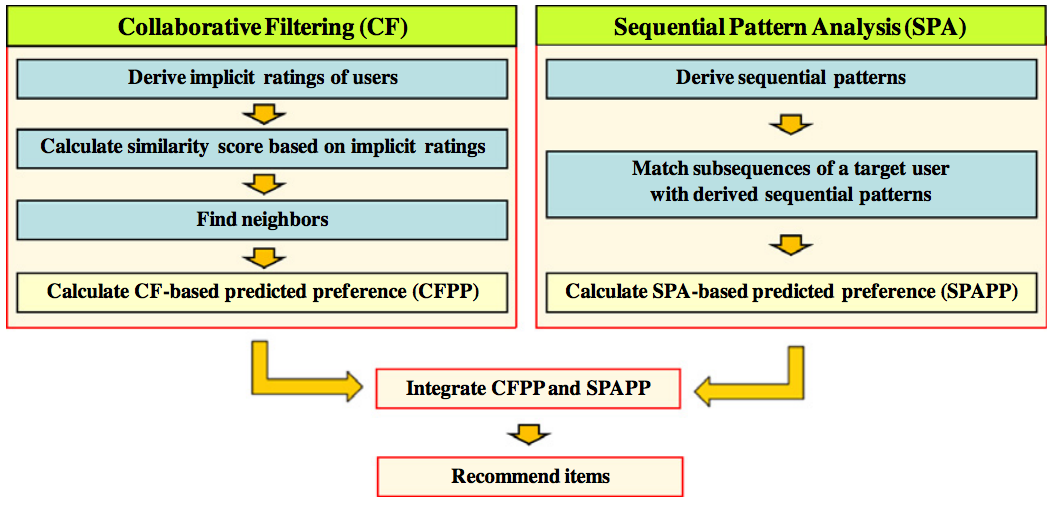
\includegraphics[scale=0.3]{image/hope-system}
  \caption{Overall framework of HOPE system, calculating implicit ratings and
  combining these with sequential pattern analysis}
  \label{hope-system}
\end{figure}

We will continue this section focusing on the convertion from transaction data
into implicit ratings, rather than going in depth into sequential pattern
analysis and calculating the CFPP and SPAPP-scores, as the interested reader
rather should consult the original research for a indepth discussion. When
calculating the $AP$ score we focus solely on the purchase data of the user
$u$, but it can easily be extended to other types of events. However, the score
does makes more sense when using it on domains having a high degree of repeated
actions - such as e-commerce stores selling convienience products with short
life spans or a music service having users listening to a song multiple times.
The absolute preference is calculated as follows:

\begin{equation}
  AP(u,i) = \ln(\frac{trans(u,i)}{\sum_{e \in E}{trans(u, e)}} + 1)
\end{equation}

where $trans(u,i)$ is the number of transactions for user $u$ on item $i$, and
E is the set of all items in our system. As an example if a user $u$ purchases an
item $i$ four times out of ten transactions the $AP(u,i) = \ln(1.4)$, but another
user $p$ who has bought the same item one time out of one transaction the
$AP(p,i) = \ln(2.0)$, and as one can see we should consider a relative preference so
that repeated actions are rewarded. Further, the absolute preference only takes
into account the frequency of purchases and because the frequency is heavily
dependent on price, item category and lifespan of an item — so in the original
research they propose the following equation in order to calcualte the relative
preference@:

\begin{equation}
  RP(u,i) = \frac{AP(u,i)}{\max_{c \in U}(AP(c,i))}
\end{equation}

where $U$ denotes every user who purchased item $i$. The reason for using a
maximization function, is to make $RP(u,i)$ range from $0.0$ to $1.0$ (i.e.\
normalization) and one can thus find a rating on a common Likert scale by
multiplying with $k$:

\begin{equation}
  ImplicitRating(u,i) = \lceil k * RP(u,i) \rceil
\end{equation}

\marginpar{todo: Do not reference ahead in the thesis. Move equation about
normalization here}
Here we round up in order to range from 1 to 5, but one could either round down
instead and have ratings range from 0 to 4 or one could use the normalization
equation defined in Equation~\ref{eq-normalization}, and setting $a = 0$ and $b
= 5$.

\subsection{Challenges and weaknesses}
\label{implicit-weaknesses}

Almost all of the research on implicit feedback has considered how behaviors
can be used as positive, rather than negative evidence. This is not to
say that we can't use user behaviors to get negative feedback, examples may
be analyzing bounce rates (e.g.\ reading an article for less than 5 seconds) or
deleting/hiding something from a feed of items. There are however much fewer of
these types of events.

Another challenge facing implicit feedback research is the notion of degree of
personalization offered by the system. In particular, individual differences
can greatly impact the effectiveness of using behavior as implicit relevance
feedback. People behave differently and have varying approaches to
information-seeking; thus, it is difficult to generate, and dangerous to apply,
all-purpose rules for describing how behavior can be used as implicit relevance
feedback.

In a classic recommender system we need three parts: ratings, a recommender
model and evaluation. Each of these parts needs to compliment each others
advantages and disadvantages. If we start top-down then we say that the
evaluation metrics used need to consider the fact that we are basing our model
on implicit ratings, and thus a preference based metric is perhaps not the best
metric (See Section~\ref{evaluation}). Further given that we choose a
precision/recall scheme then we need to choose good parameters showing both the
strengths and weaknesses found in the data and recommender model. How many
recommendations should we provide the user in order to calculate precision and
recall? And which metrics should we focus on; F1; MPR or others?
\marginpar{Are MPR and F1 introduced?} 
When considering the recommender model there are as many countless
possibibilites - ranging from traditional approcahes such as
Pearson-correlation and K-nearest neighbours to more advanced and perhaps more
specialized approaches such as SVD++. A common theme when using more advanced
models are the number of parameters available for adjustments increases almost
linearily. In a simple KNN-approach we can get various results by varying K -
whilst in SVD++ we can vary the learning rate, alpha, number of features and
many others~\ref{svdplusplus}. The approach we use in order to create our
recommender model should consider the \textit{type} of ratings (explicit or
implicit), the sparsity, the domain, number of items vs. number of users and
many others. And lastly when we are creating ratings we should, as this section
has mentioned several times, choose an approach matching the domain - as there
can be large differences between e.g.\ an online TV-streaming service and an
E-commerce store selling fashion.

%TODO: Helge sier:
% I mitt hode skal det optimeres ut fra datatilgang (om det er statisk) eller
% beslutingsproblem. Ikke god forskning å velge evaluering ut fra metodevalg.

This large choice of different models and their parameters in all stages from
generation of ratings to evaluation, makes the pipeline quite vulnerable to
fluxuations in results by small adjustments early in the pipeline. That is, by
adjusting parameters in our first stage (generation of implicit ratings) it can
have great effects on both our mathematical model and evaluation metrics. The
number of different approaches makes it difficult to effectivly show all
possibilites to the user and for some domains, even those focused on in this
paper, it would not make sense to test some models or metrics.

% \todo{Mention fashion-specific challenges, e.g.\ clicks does not equal high
% rating}
When considering the domain of e-commerce websites a common approach is to both
count transactions and clicks~\cite{something}, but ...

% \todo{Add weaknesses of explicit ratings}

% \subsection{Evaluating conversion to implicit ratings}

% Map against user study.

% Refer to evaluation section, written by Martin.
